\chapter{Spezifikation des zu entwerfenden Systems in Text und Bild}

\section{Erläuterung der Aufgabe}
Zur Implementierung des SPI-Slaves sind folgende Entwurfsschritte von nöten:
\begin{itemize}
  \item algorithmische Ebene
  \begin{itemize}
    \item Entwurf eines VHDL-Modells auf algorithmischer Ebene mit zugehöriger Testbench
    \item Funktionale Simulation der algorithmischen Ebene
  \end{itemize}
  \item Register Transfer Ebene
  \begin{itemize}
    \item Entwurf eines VHDL-Modells auf Register Transfer Ebene mit zugehöriger Testbench
    \item Funktionale Simulation der RT-Ebene vs. algorithmischer Ebene
    \item Timing Simulation des Ergebnises
  \end{itemize}
  \item Die Realisierung muss auf dem DE2-Evaluierungsboard lauffähig sein
\end{itemize}

\section{Beschreibung der Ein- und Ausgänge}
\begin{figure}[ht]
    \centering
    \vspace{-1em}
        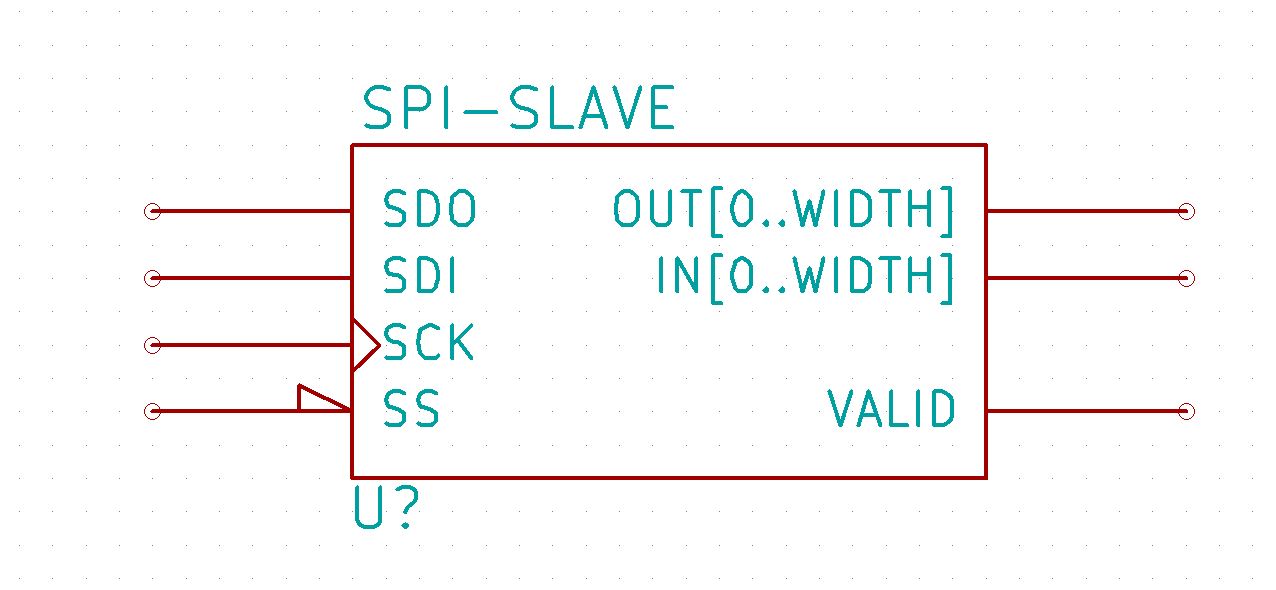
\includegraphics[width=0.9\textwidth]{img/SLAVE.png}
    \vspace{-1em}    
    \caption{Blockschaltbild des Slaves (ohne generische Parameter)}
    \label{fig:blockSlave}
\end{figure}
\newpage
Es existieren drei gemeinsame Leitungen, an denen jeder Teilnehmer angeschlossen ist:
\begin{itemize}
  \item [SDO] (englisch Serial Data Out) bzw. MISO oder SOMI (englisch Master in, Slave out)
  \item [SDI] (englisch Serial Data In) bzw. MOSI oder SIMO (englisch Master out, Slave in)
  \item [SCK] (englisch Serial Clock) bzw. SCLK, wird vom Master ausgegeben
  \item [OUT] ''Ausgaberegeister'' Parallele Ausgänge des Ausgangswort, je nach Wortbreite über
              \emph{generic} parametrisiert
  \item [IN]  ''Eingangsregeister'' Parallele Eingänge, je nach Wortbreite über
              \emph{generic} parametrisiert
  \item [VALID] Ausgang, welcher einen Impuls(halbe Periodenbreite) generiert wenn das Eingangswort
              gültig ist
\end{itemize}

Eine logisch-0 aktive Chip-Select-Leitungen, welche vom Master gesteuert wird. Diese Leitung wird je
nach Anwendung unterschiedlich mit Bezeichnungen wie SS, CS oder STE für Slave Select, Chip Select bzw.
Slave Transmit Enable bezeichnet, oft noch in Kombination mit einer Indexnummer zur Unterscheidung.
Es gibt auch spezielle Anwendungen, bei denen sich mehrere Slaves diese Leitung teilen. Viele
Einstellmöglichkeiten, beispielsweise mit welcher Taktflanke ausgegeben bzw. eingelesen wird,
Wortlänge, Übertragung MSB oder LSB zuerst.

Viele Einstellungsmöglichkeiten sind unter anderem deshalb erforderlich, weil sich die Spezifikation
für den SPI-Bus in vielen Dingen nicht konkret festlegt und deshalb verschiedene, zueinander
inkompatible Geräte existieren. So ist häufig für jeden angeschlossenen Schaltkreis eine eigene
Konfiguration des steuernden Mikrocontrollers (Master des SPI-Bus) erforderlich.

Es können theoretisch beliebig viele Teilnehmer an den Bus angeschlossen werden, wobei es immer
genau einen Master geben muss. Er ist derjenige, der das Clock-Signal an SCK erzeugt und festlegt,
mit welchem Slave er kommunizieren will. Das geschieht über die Leitung ''Slave Select''. Wird sie
gegen Masse gezogen, wird der jeweilige Slave aktiv, ''lauscht'' an MOSI und legt seine Daten im
Takt von SCK an MISO. Es wird somit ein Byte vom Master zum Slave und ein anderes Byte vom Slave zum
Master transportiert.

Ein Protokoll für die Datenübertragung wurde von Motorola zwar nicht festgelegt, doch haben sich in
der Praxis vier verschiedene Modi durchgesetzt. Diese werden durch die Parameter Clock Polarität
(CPOL) und Clock Phase (CPHA) festgelegt. Bei CPOL=0 ist der Clock Idle Low, bei CPOL=1 ist der
Clock Idle High. CPHA gibt nun an, bei der wievielten Flanke die Daten übernommen werden sollen. Bei
CPHA=0 werden sie bei der ersten Flanke übernommen, nachdem SS auf Low gezogen wurde, bei CPHA=1 bei
der zweiten. Somit werden die Daten bei CPOL=0 und CPHA=0 mit der ersten Flanke übernommen, die nur
eine High-Flanke sein kann. Bei CPHA=1 wäre es die zweite, also eine Low-Flanke. Bei CPOL=1 ist das
ganze folglich genau andersherum, bei CPHA=0 Low-Flanke und bei CPHA=1 High-Flanke.

Zu beachten ist noch, dass der Slave bei CPHA=0 seine Daten schon beim Runterziehen von SS an MISO
anlegt, damit der Master sie beim ersten Flankenwechsel übernehmen kann. Bei CPHA=1 werden die Daten
vom Slave erst beim ersten Flankenwechsel an MISO gelegt, damit sie beim zweiten Flankenwechsel vom
Master übernommen werden können. Der Master hingegen legt seine Daten immer zum gleichen Zeitpunkt
an, meist kurz nach der Low-Flanke von SCK.

Mit jeder Taktperiode wird ein Bit übertragen. Beim üblichen Bytetransfer sind also 8 Taktperioden
für eine vollständige Übertragung nötig. Es können auch mehrere Bytes hintereinander übertragen
werden, wobei nicht festgelegt ist, ob zwischen jedem Byte das SS-Signal kurz wieder auf High
gezogen werden muss. Eine Übertragung ist beendet, wenn das Slave-Select-Signal endgültig auf High
gesetzt wird.

\vspace{1em}
\begin{table}[h]
  \centering
  \begin{tabular}{| l || c | r |}
  \hline                        
  Mode & CPOL & CPHA \\
  \hline                        
  0 & 0 & 0 \\
  1 & 0 & 1 \\
  2 & 1 & 0 \\
  3 & 1 & 1 \\
  \hline  
  \end{tabular}
  \caption{Übersicht der verschiedenen Modi}
  \label{tab:modes}
\end{table}
\vspace{1em}
\begin{figure}[ht]
    \centering
    \vspace{-1em}
        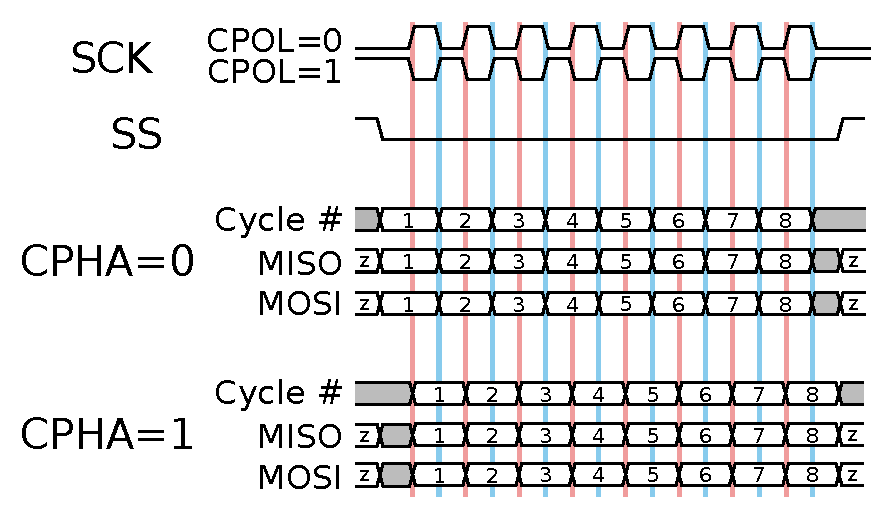
\includegraphics[width=0.9\textwidth]{img/SPItiming.pdf}
    \vspace{-1em}    
    \caption{Timing Diagramm zum SPI Protokoll}
    \label{fig:timing}
\end{figure}

\section{use-Cases}
Da eine genaue Wortbreite in der Spezifikation nicht vorgegeben ist, wird im folgendem von einem
8Bit breitem Datenwort ausgegangen.
Mögliche use-Cases sind:
\begin{itemize}
  \item Ein Datenwort empfangen/senden
  \item n Datenworte empfangen/senden
  \item fehlerhaftes Datenwort empfangen/senden
  \item n fehlerhafte Datenworte empfangen/senden
\end{itemize}

Diese sollten in allen vier Modi abgedeckt werden (siehe Tabelle \ref{tab:modes}).

\section{Lösungsansatz}
Nach dem Entwurf auf algorithmischer Ebene, wird das Modell mit der entsprechenden Testbench
verifiziert. Ist dieder Test erfolgreich, so ist ein Signalübergangsgraph zu entwerfen und aus Ihm
mit einer geeigneten Entwurfsmethode ein oder mehrere Automaten (Mealy/Moore/FSMD) abzuleiten.
Diese Realisierung ist wieder mit einer Testbench zu verifizieren (cycle accurate) und auf dem
DE2-Evaluationsboard zu implementieren.
